\documentclass[12pt]{article}

\usepackage[utf8]{inputenc}
\usepackage[T1]{fontenc}
\usepackage[polish,provide=*]{babel}
\usepackage{lmodern}
\usepackage{amsmath}
\usepackage{latexsym,amsfonts,amssymb,amsthm,amsmath}
\usepackage{enumitem}
\usepackage{float}
\usepackage{hyperref}
\usepackage{graphicx}
\usepackage{subcaption}
\usepackage{booktabs}
\graphicspath{{./images/}}

\setlength{\parindent}{0in}
\setlength{\oddsidemargin}{0in}
\setlength{\textwidth}{6.5in}
\setlength{\textheight}{8.8in}
\setlength{\topmargin}{0in}
\setlength{\headheight}{18pt}

\title{Badanie spektrum lampy RGB}
\author{Kacper Kłos}

\begin{document}
\maketitle

Niniejszy raport przedstawia wyniki badania spektrum lampy RGB za pomocą zbudowanego przez nas spektrometru.  
Układ pomiarowy składał się z trzech soczewek, szczeliny oraz siatki dyfrakcyjnej.  
Pierwszy rząd widma skierowaliśmy na detektor, który pozwalał dokładnie wyznaczyć natężenie światła w zależności od położenia.  
Dodatkowo widmo źródła zmierzono spektrometrem komercyjnym, aby określić dokładne długości fal emitowanych przez lampę.

\vspace{1 in}

\section{Wyniki pomiarów}

Wszystkie dane znajdują się w dwóch załączonych plikach.  
Plik \textit{spektrometr.csv} zawiera wyniki uzyskane spektrometrem komercyjnym, a \textit{detektor.csv} – pięć serii pomiarowych wykonanych detektorem natężenia.  
W raporcie analizujemy jedynie dwie ostatnie serie, gdyż wcześniejsze dotyczyły kalibracji spektrometru.

Widmo zmierzone spektrometrem komercyjnym przedstawiono na rysunku~\ref{fig:spektrometr}.

\begin{figure}[H]
  \centering
  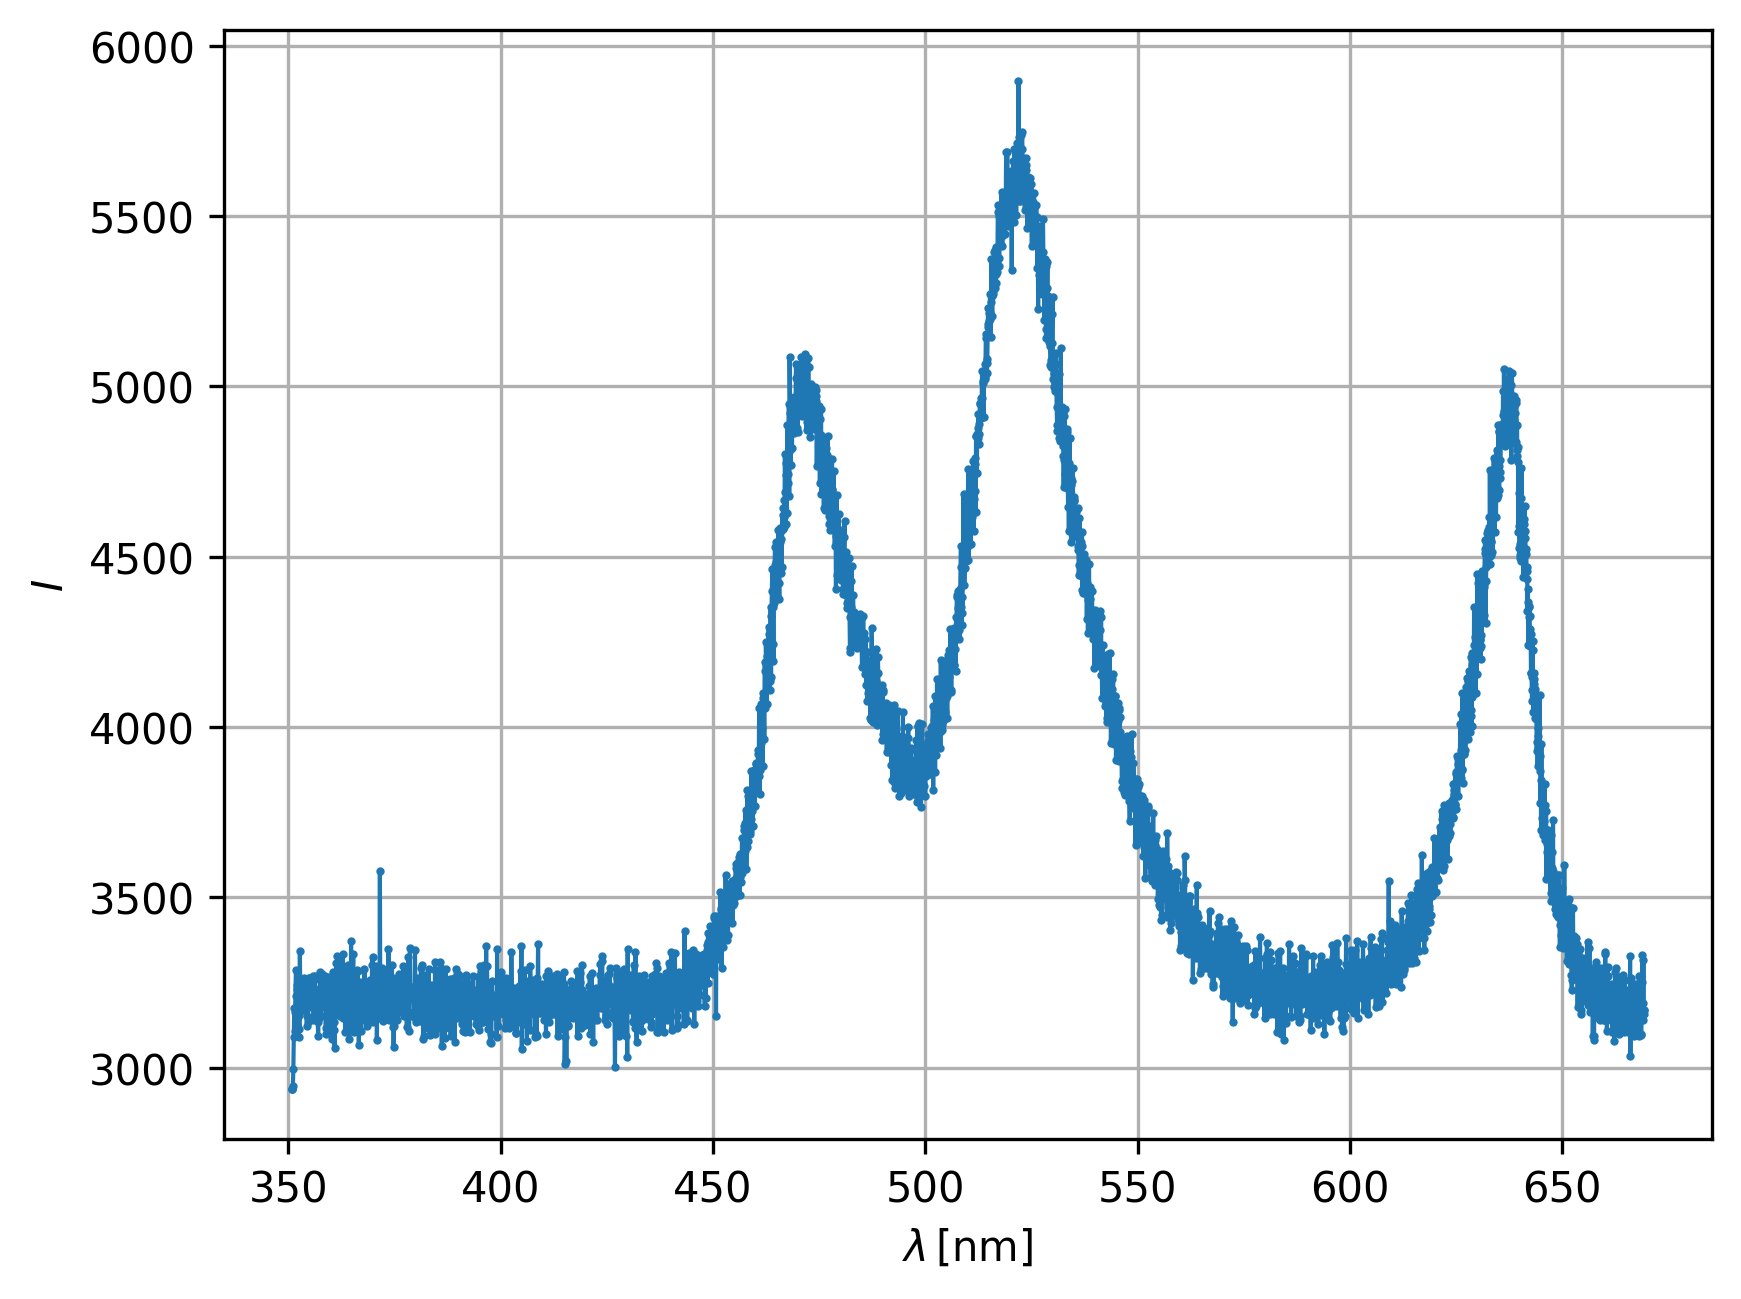
\includegraphics[scale=0.7]{spektrum}
  \caption{Widmo lampy RGB zarejestrowane spektrometrem Flame-T (Ocean Insight).}
  \label{fig:spektrometr}
\end{figure}

Na wykresie widać trzy wyraźne maksimum, dla których otrzymaliśmy  

\[
  \lambda_{\mathrm{blue}} = (472 \pm 6)\,\mathrm{nm}, \quad
  \lambda_{\mathrm{green}} = (522 \pm 3)\,\mathrm{nm}, \quad
  \lambda_{\mathrm{red}}  = (636 \pm 4)\,\mathrm{nm}.
\]

Niepewność określono jako największą różnicę między długością fali w maksimum a wartościami mieszczącymi się w \(95\%\) maksymalnej intensywności.

\subsection*{Pomiary detektorem}

Dane z detektora spektrometru własnej konstrukcji przedstawiono na rysunku~\ref{fig:detektor}.

\begin{figure}[H]
  \centering
  \begin{subfigure}{0.45\textwidth}
    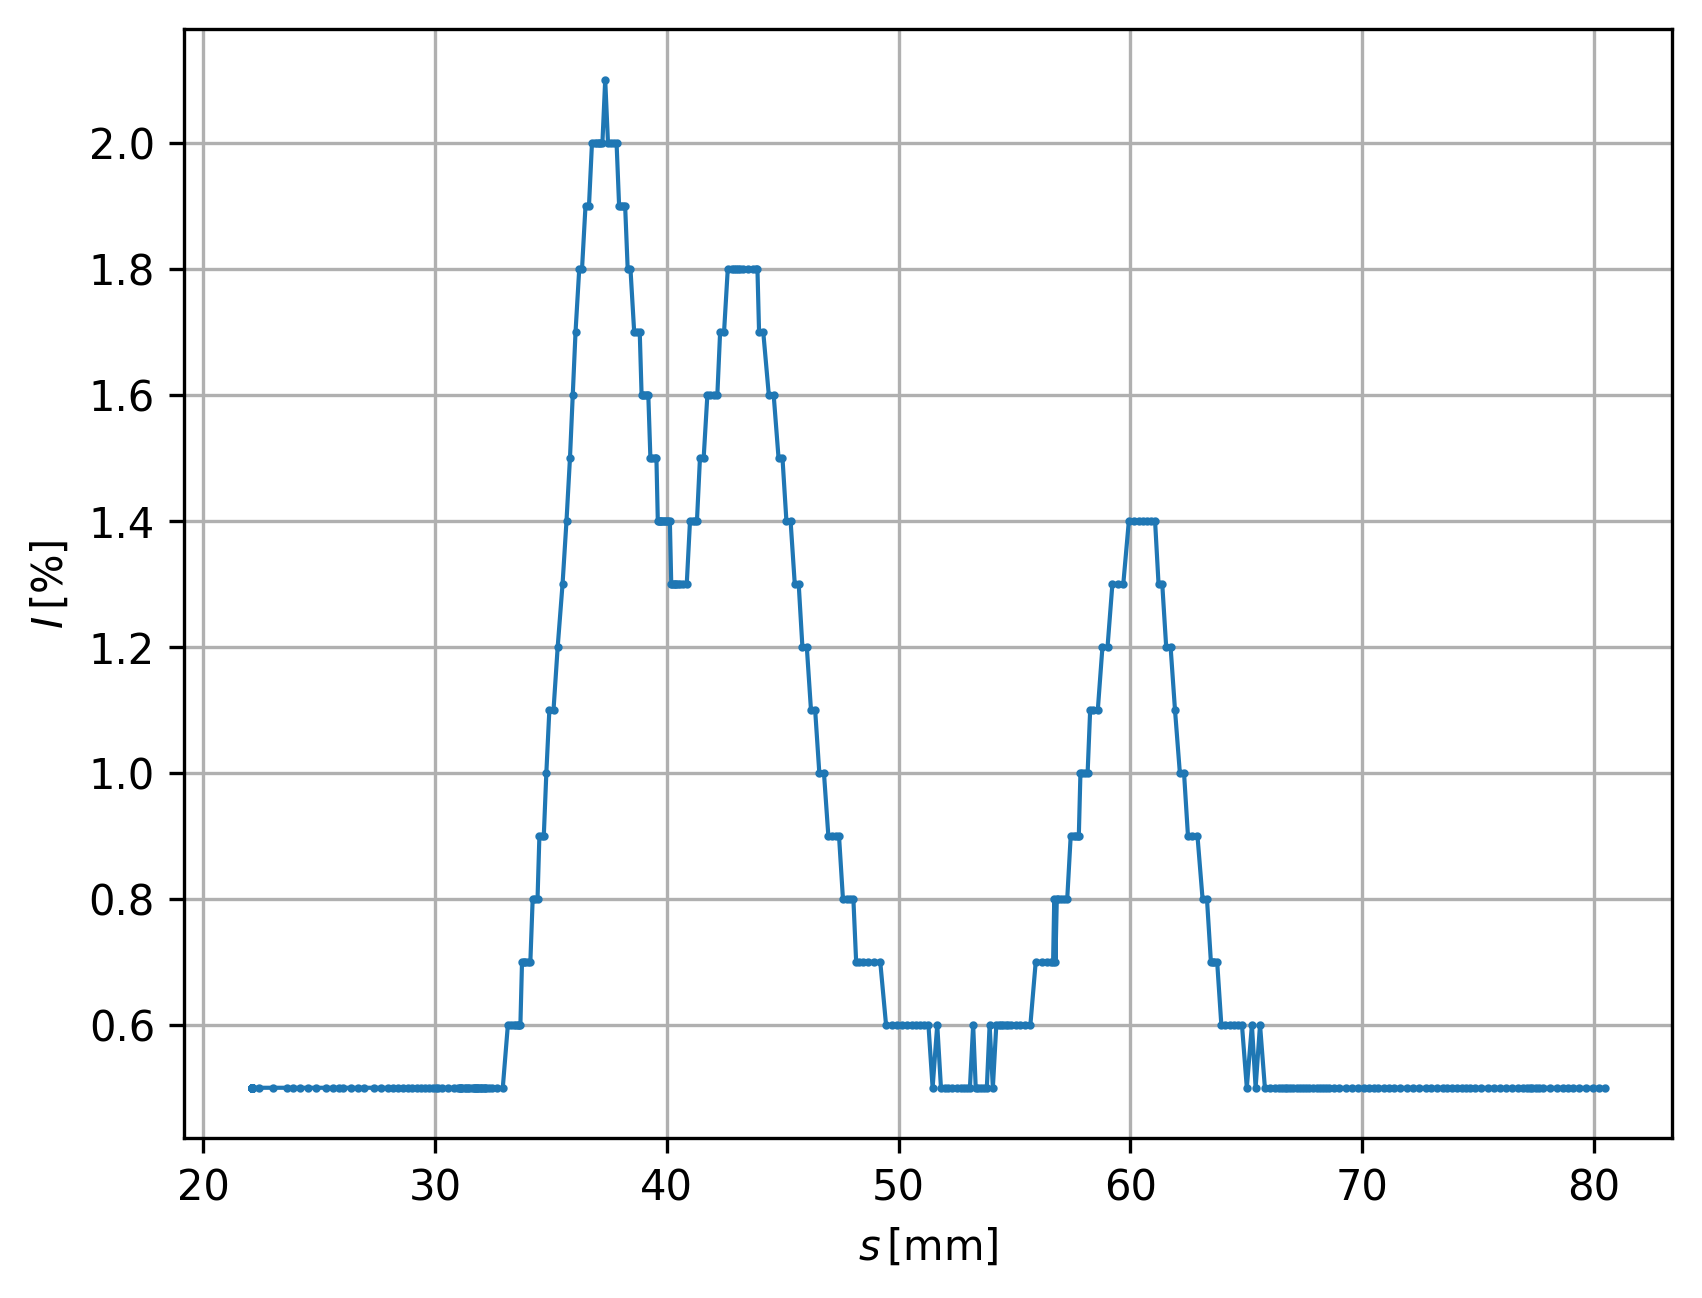
\includegraphics[width=\linewidth]{detektor0}
    \caption{seria 1}
    \label{fig:detektor_1}
  \end{subfigure}\hfill
  \begin{subfigure}{0.45\textwidth}
    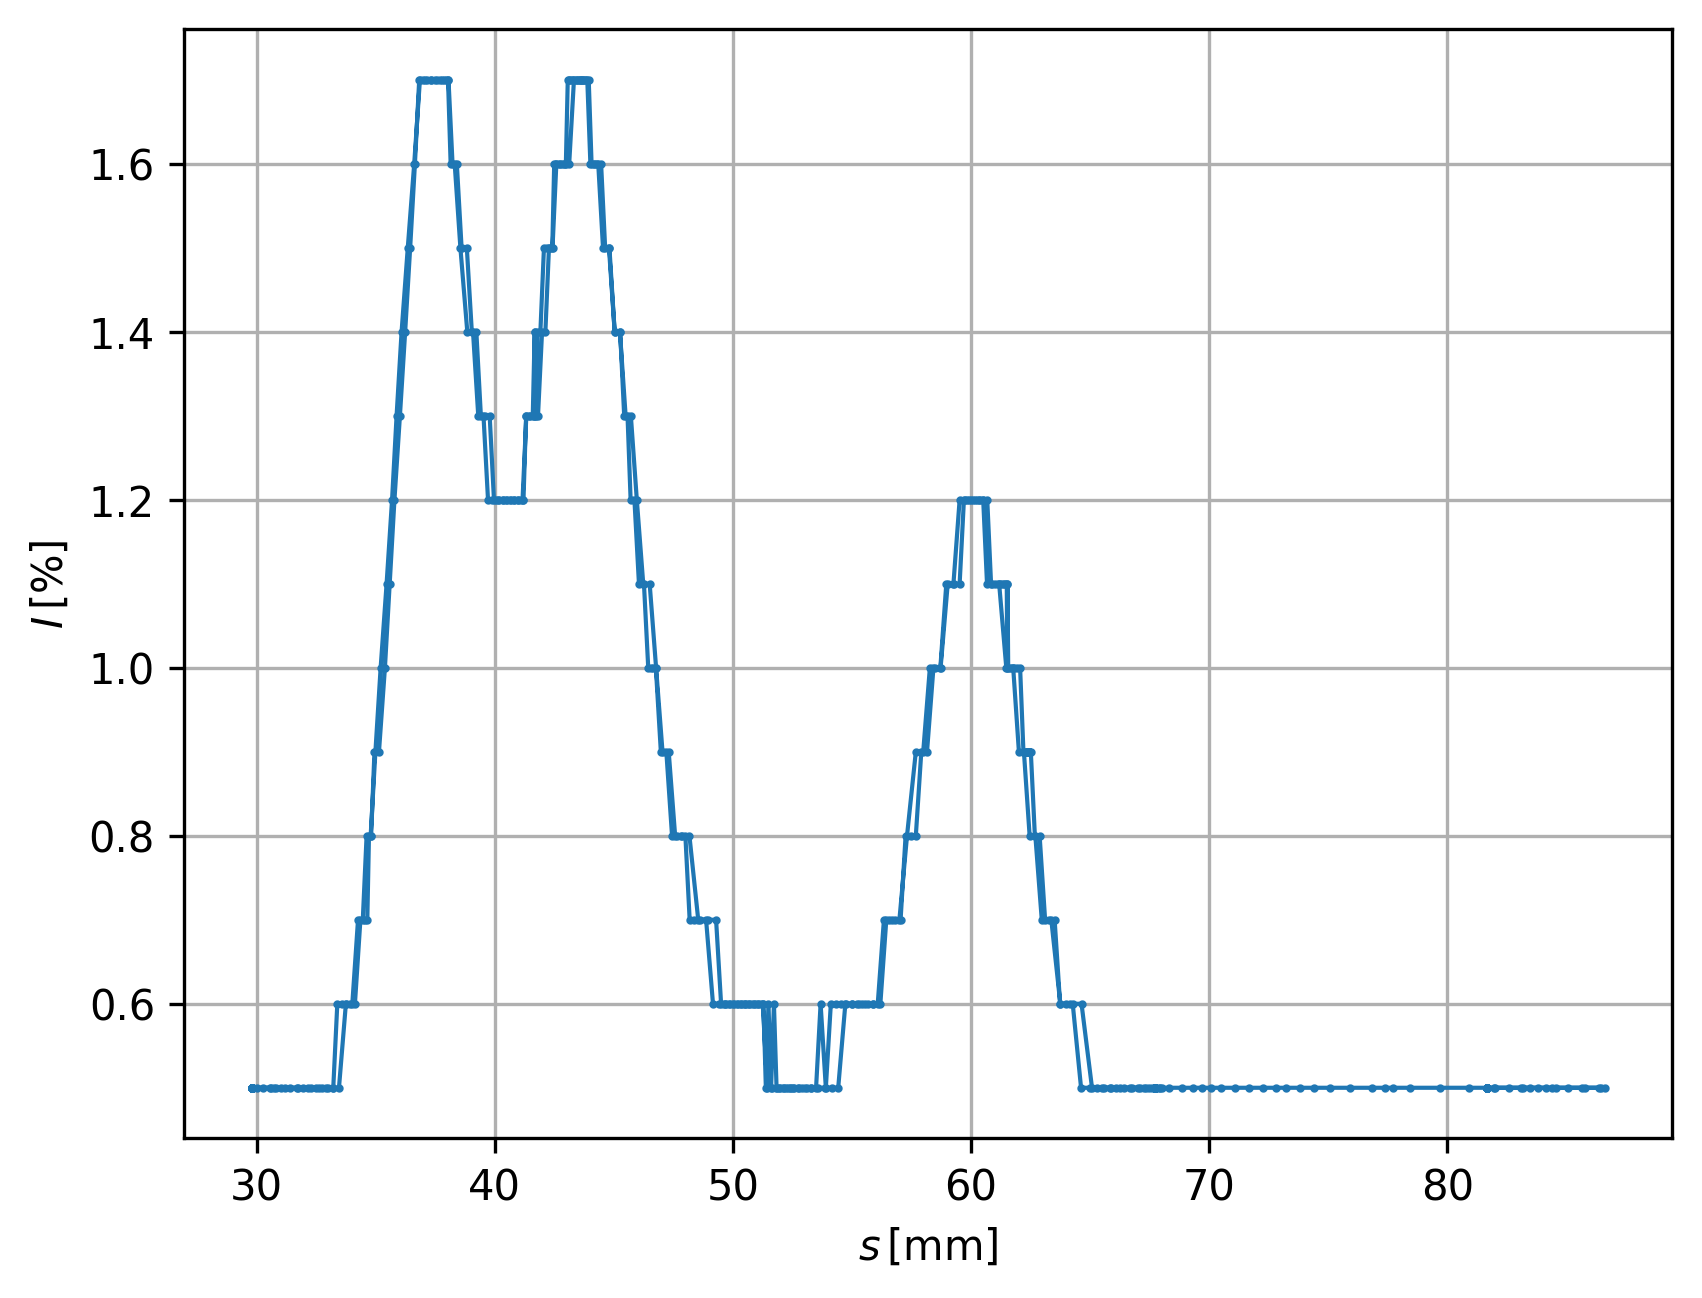
\includegraphics[width=\linewidth]{detektor1}
    \caption{seria 2}
    \label{fig:detektor_2}
  \end{subfigure}
  \caption{Natężenie światła w funkcji położenia detektora PASCO OS-8441.}
  \label{fig:detektor}
\end{figure}

Kształt widma odpowiada wynikowi spektrometru komercyjnego. Drobne różnice w kształcie intensywności mogą wynikać z absorpcji elementów optycznych, nieidealnego ustawienia soczewki skupiającej promienie na detektorze lub mniejszej precyzji.

\paragraph{Seria 1 (rys.~\ref{fig:detektor_1})}
\[
  y_{\mathrm{blue}}  = (37{,}34 \pm 0{,}57)\,\mathrm{mm}, \quad
  y_{\mathrm{green}} = (42{,}63 \pm 1{,}53)\,\mathrm{mm}, \quad
  y_{\mathrm{red}}   = (59{,}94 \pm 1{,}44)\,\mathrm{mm}.
\]

\paragraph{Seria 2 (rys.~\ref{fig:detektor_2})}
\[
  y_{\mathrm{blue}}  = (38{,}03 \pm 1{,}21)\,\mathrm{mm}, \quad
  y_{\mathrm{green}} = (43{,}88 \pm 0{,}82)\,\mathrm{mm}, \quad
  y_{\mathrm{red}}   = (60{,}51 \pm 0{,}99)\,\mathrm{mm}.
\]

Niepewności wyznaczono jako największą różnicę między położeniem maksimum a pozycjami, w których intensywność spada odpowiednio do \(90\%\) (seria 1) i \(95\%\) (seria 2) wartości maksymalnej. Mniejszy błąd w drugiej serii wynika z dwukrotnego przejazdu detektora w obie strony.

\subsection*{Kalibracja zależności \(\lambda(y)\)}

Zgodnie z~\cite{skrypt} przyjęto zależność liniową  

\[
  \lambda = a\,y + b.
\]

\begin{figure}[H]
  \centering
  \begin{subfigure}{0.45\textwidth}
    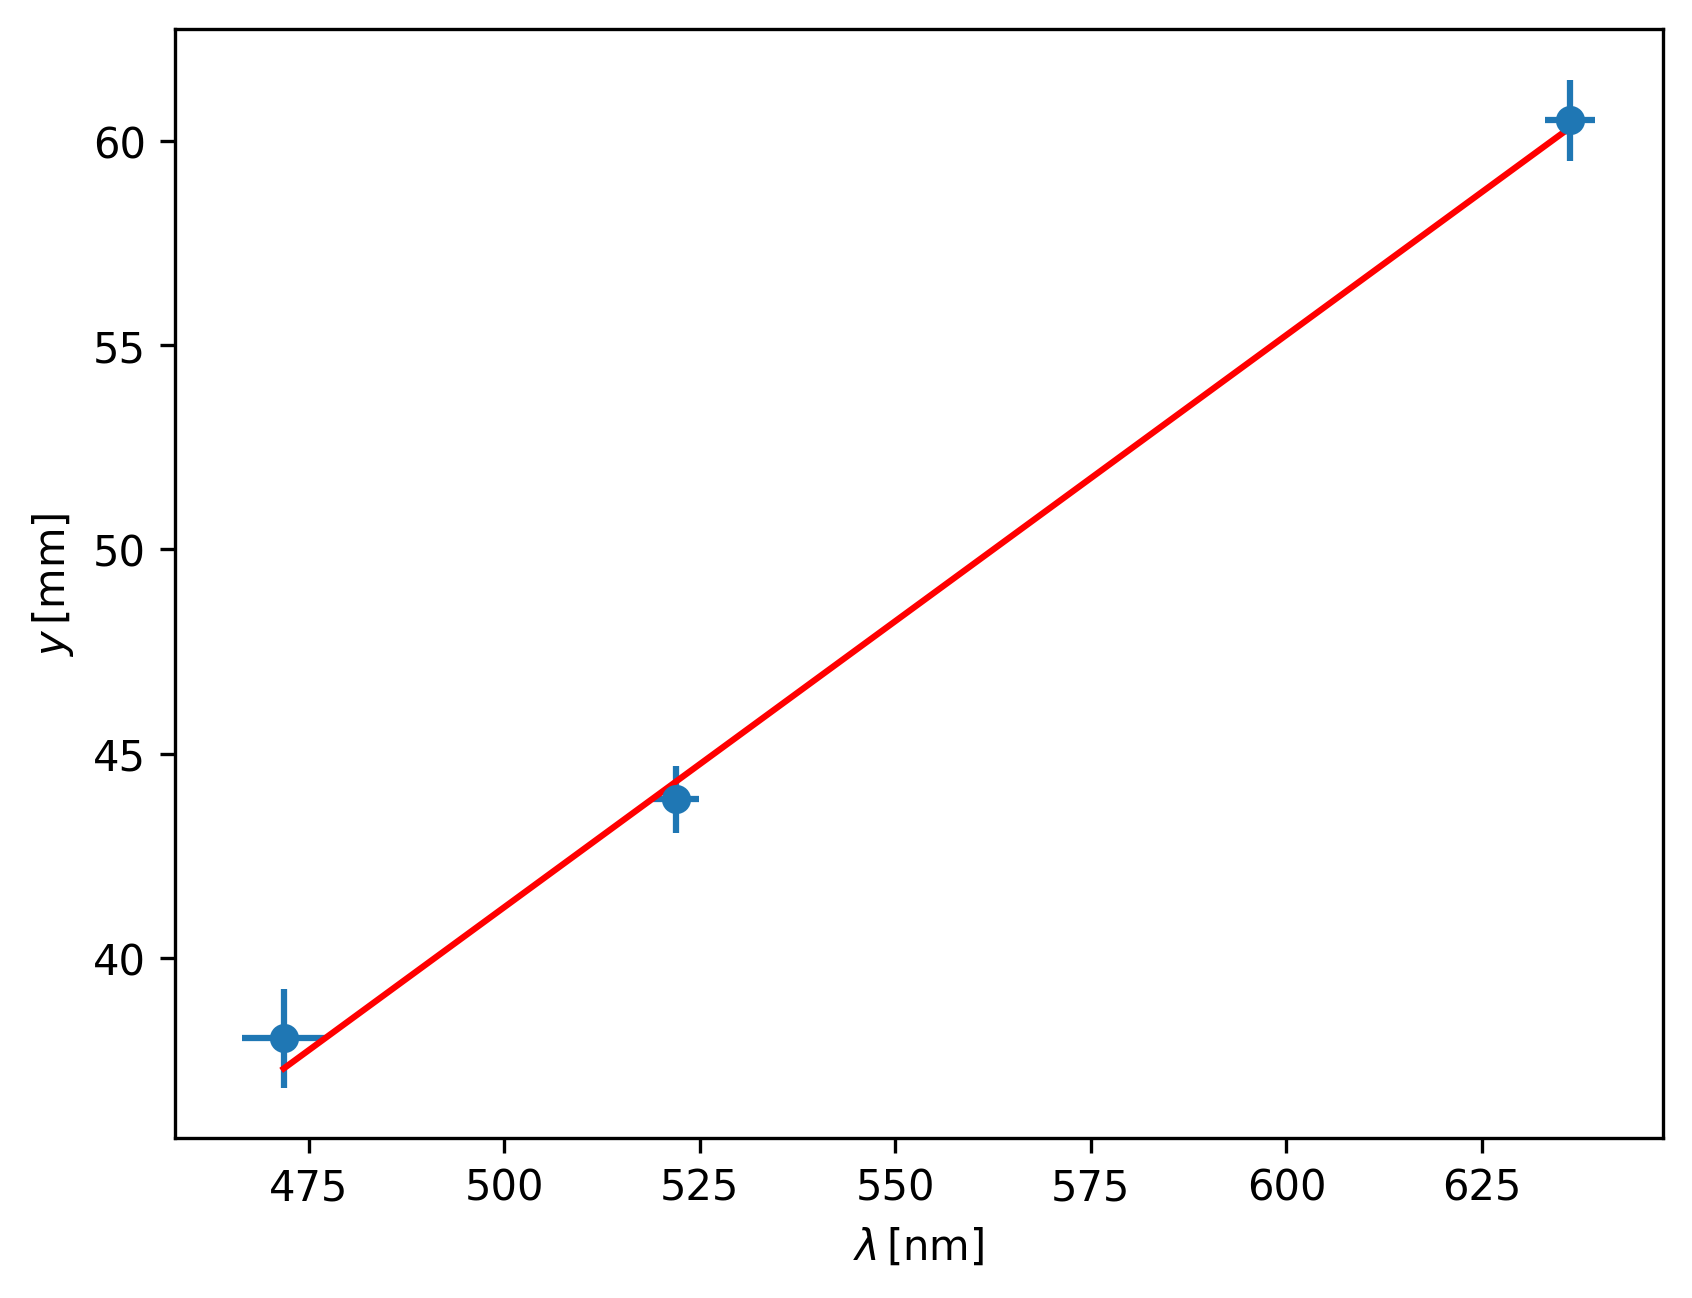
\includegraphics[width=\linewidth]{line_fit_distance_1}
    \caption{seria 1}
    \label{fig:line_fit_distance_1}
  \end{subfigure}\hfill
  \begin{subfigure}{0.45\textwidth}
    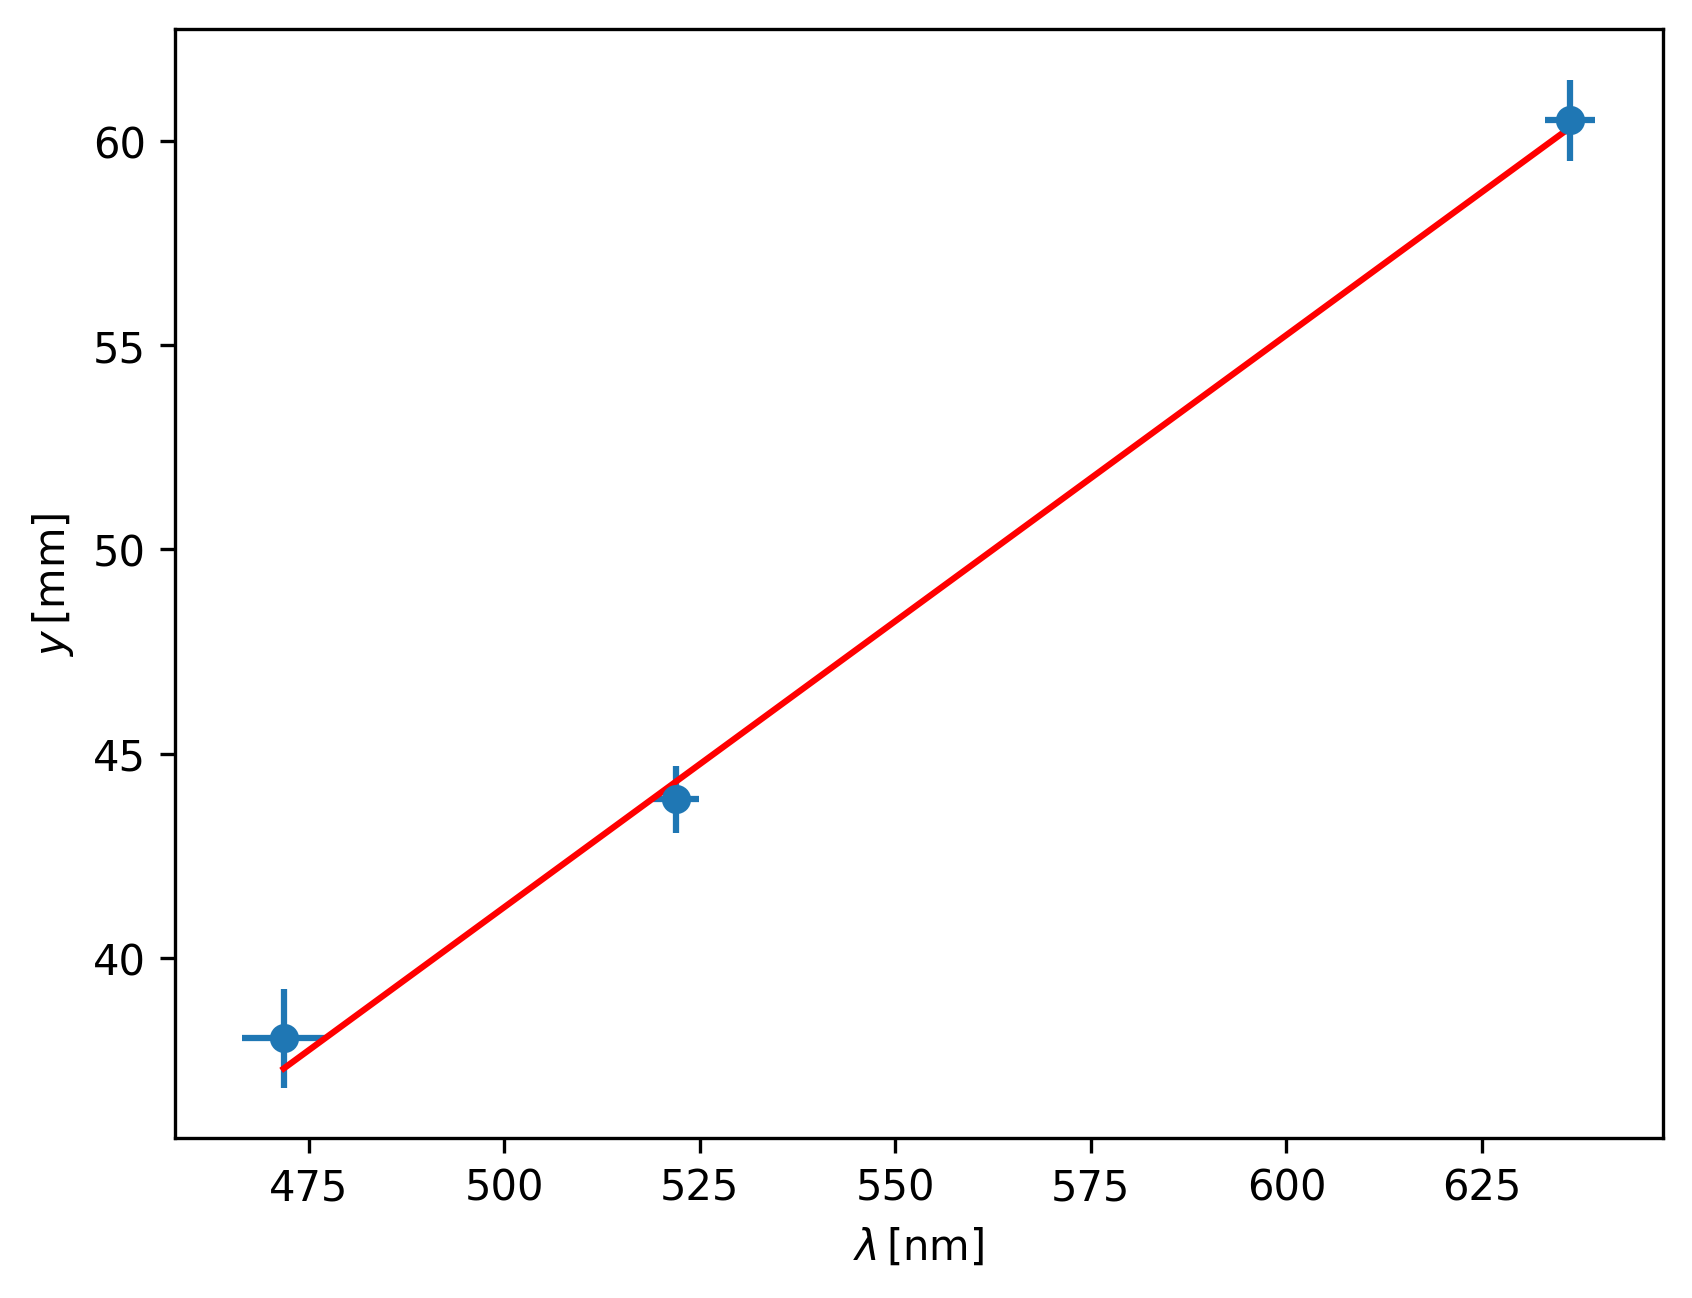
\includegraphics[width=\linewidth]{line_fit_distance_1}
    \caption{seria 2}
    \label{fig:line_fit_distance_2}
  \end{subfigure}
  \caption{Dopasowanie liniowe \(\lambda(y)\).}
  \label{fig:line_fit_distance}
\end{figure}

\textbf{Seria 1 (rys.~\ref{fig:line_fit_distance_1}):}  
\(a = (1{,}37 \pm 0{,}10) \times 10^{5}, \quad b = (-28 \pm 6)\,\mathrm{mm},\)

\[
  \text{macierz kowariancji} =
  \begin{bmatrix}
    9{,}6224 \times 10^{7} & -4{,}9873 \times 10^{1}\,\mathrm{m}^2 \\
    -4{,}9873\times 10^{1}\,\mathrm{m}^2 & 2{,}6257 \times 10^{-5}\,\mathrm{m}^2
  \end{bmatrix}.
\]

\textbf{Seria 2 (rys.~\ref{fig:line_fit_distance_2}):}  
\(a = (1{,}40 \pm 0{,}08) \times 10^{5}, \quad b = (-29 \pm 4)\,\mathrm{nm},\)

\[
  \text{macierz kowariancji} =
  \begin{bmatrix}
      5{,}1632 \times 10^{7} & -2{,}8408\times10^{1}\,\mathrm{m} \\
    -2{,}8408\times10^{1}\,\mathrm{m} & 1{,}5838\times10^{-5}\,\mathrm{m}^2
  \end{bmatrix}.
\]

Średnia ważona daje  
\[
  \bar{a} = (1{,}39 \pm 0{,}06) \times 10^{5}, \quad
  \bar{b} = (-28 \pm 4)\,\mathrm{mm}.
\]

\subsection*{Kalibracja odwrotna \(y(\lambda)\)}

Rozważono także zależność odwrotną  

\[
  y = A\,\lambda + B.
\]

\begin{figure}[H]
  \centering
  \begin{subfigure}{0.45\textwidth}
    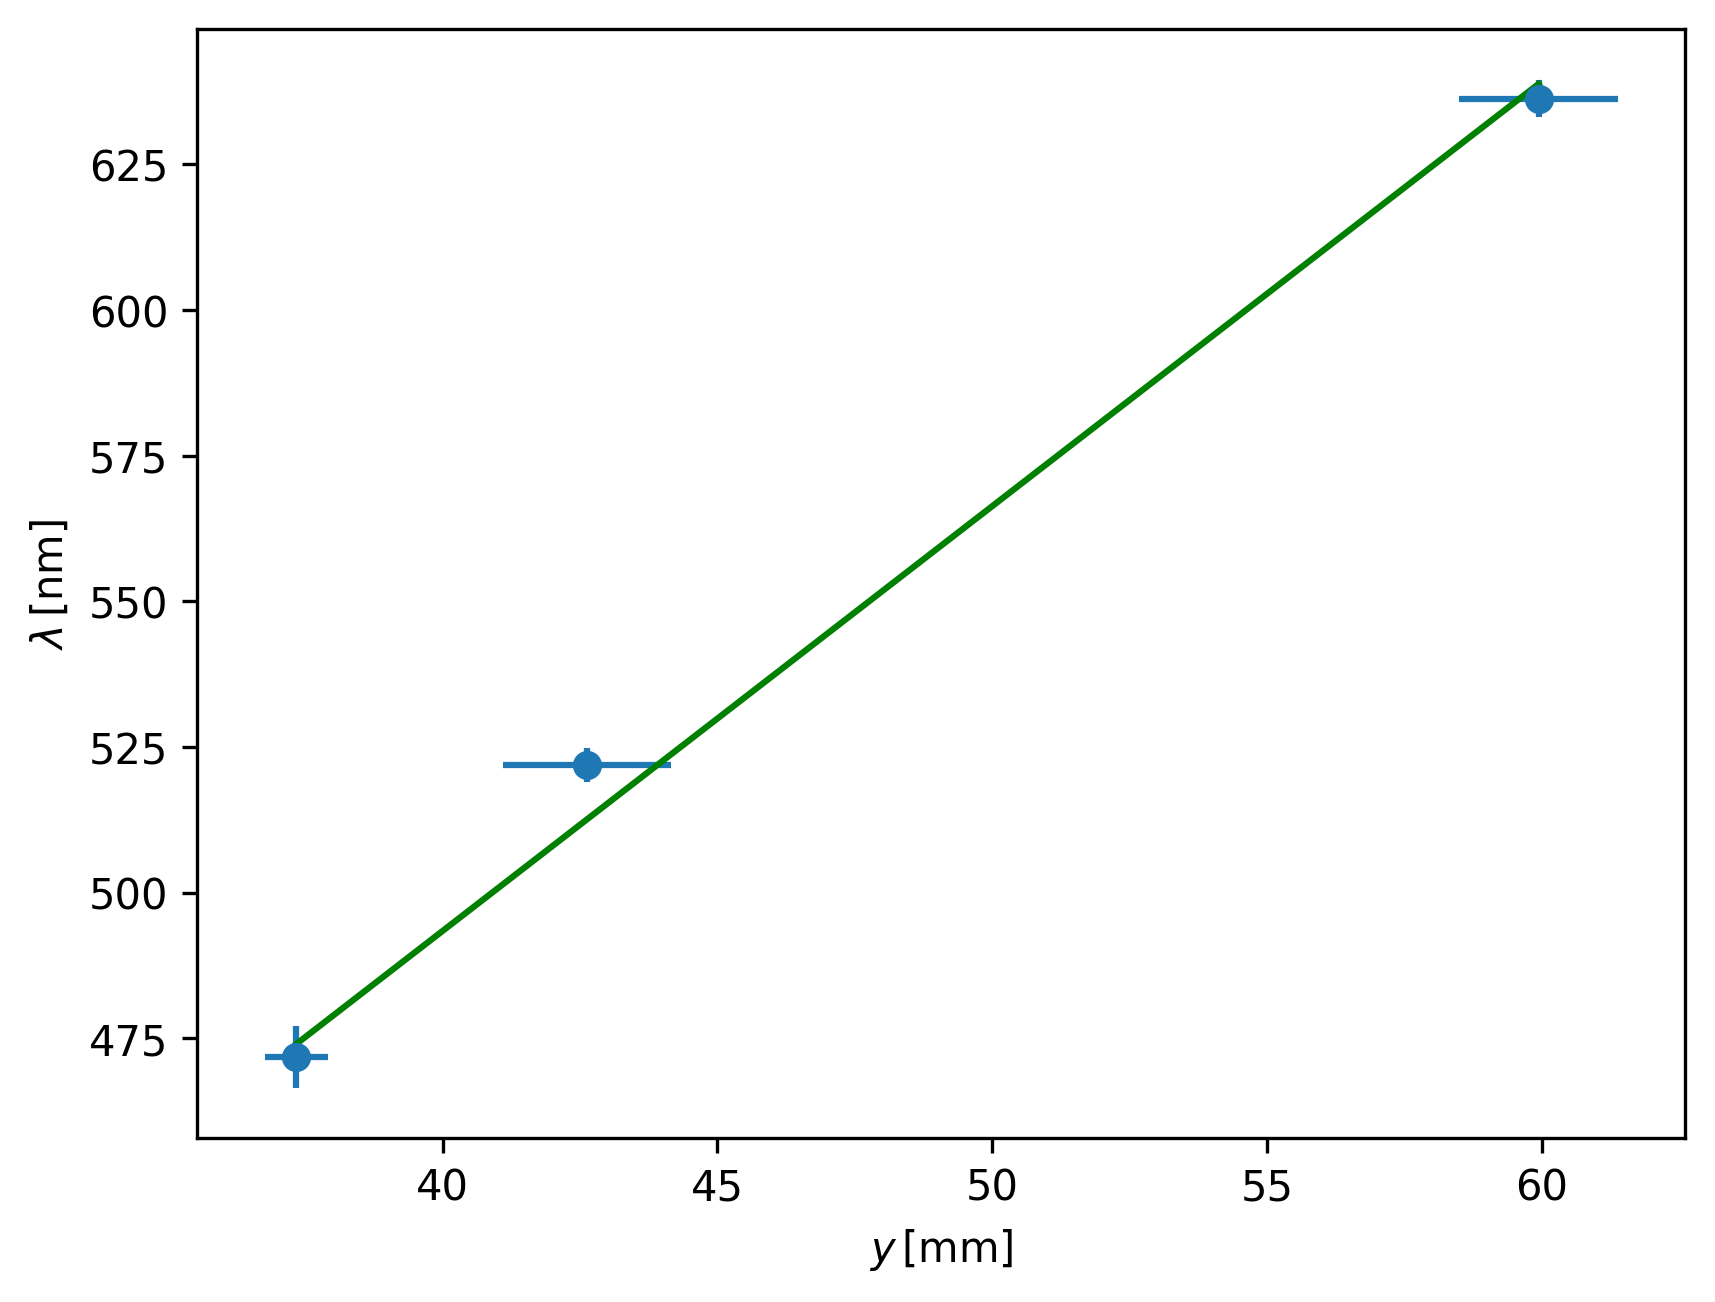
\includegraphics[width=\linewidth]{line_fit_wavelength_0}
    \caption{seria 1}
    \label{fig:line_fit_wavelength_1}
  \end{subfigure}\hfill
  \begin{subfigure}{0.45\textwidth}
    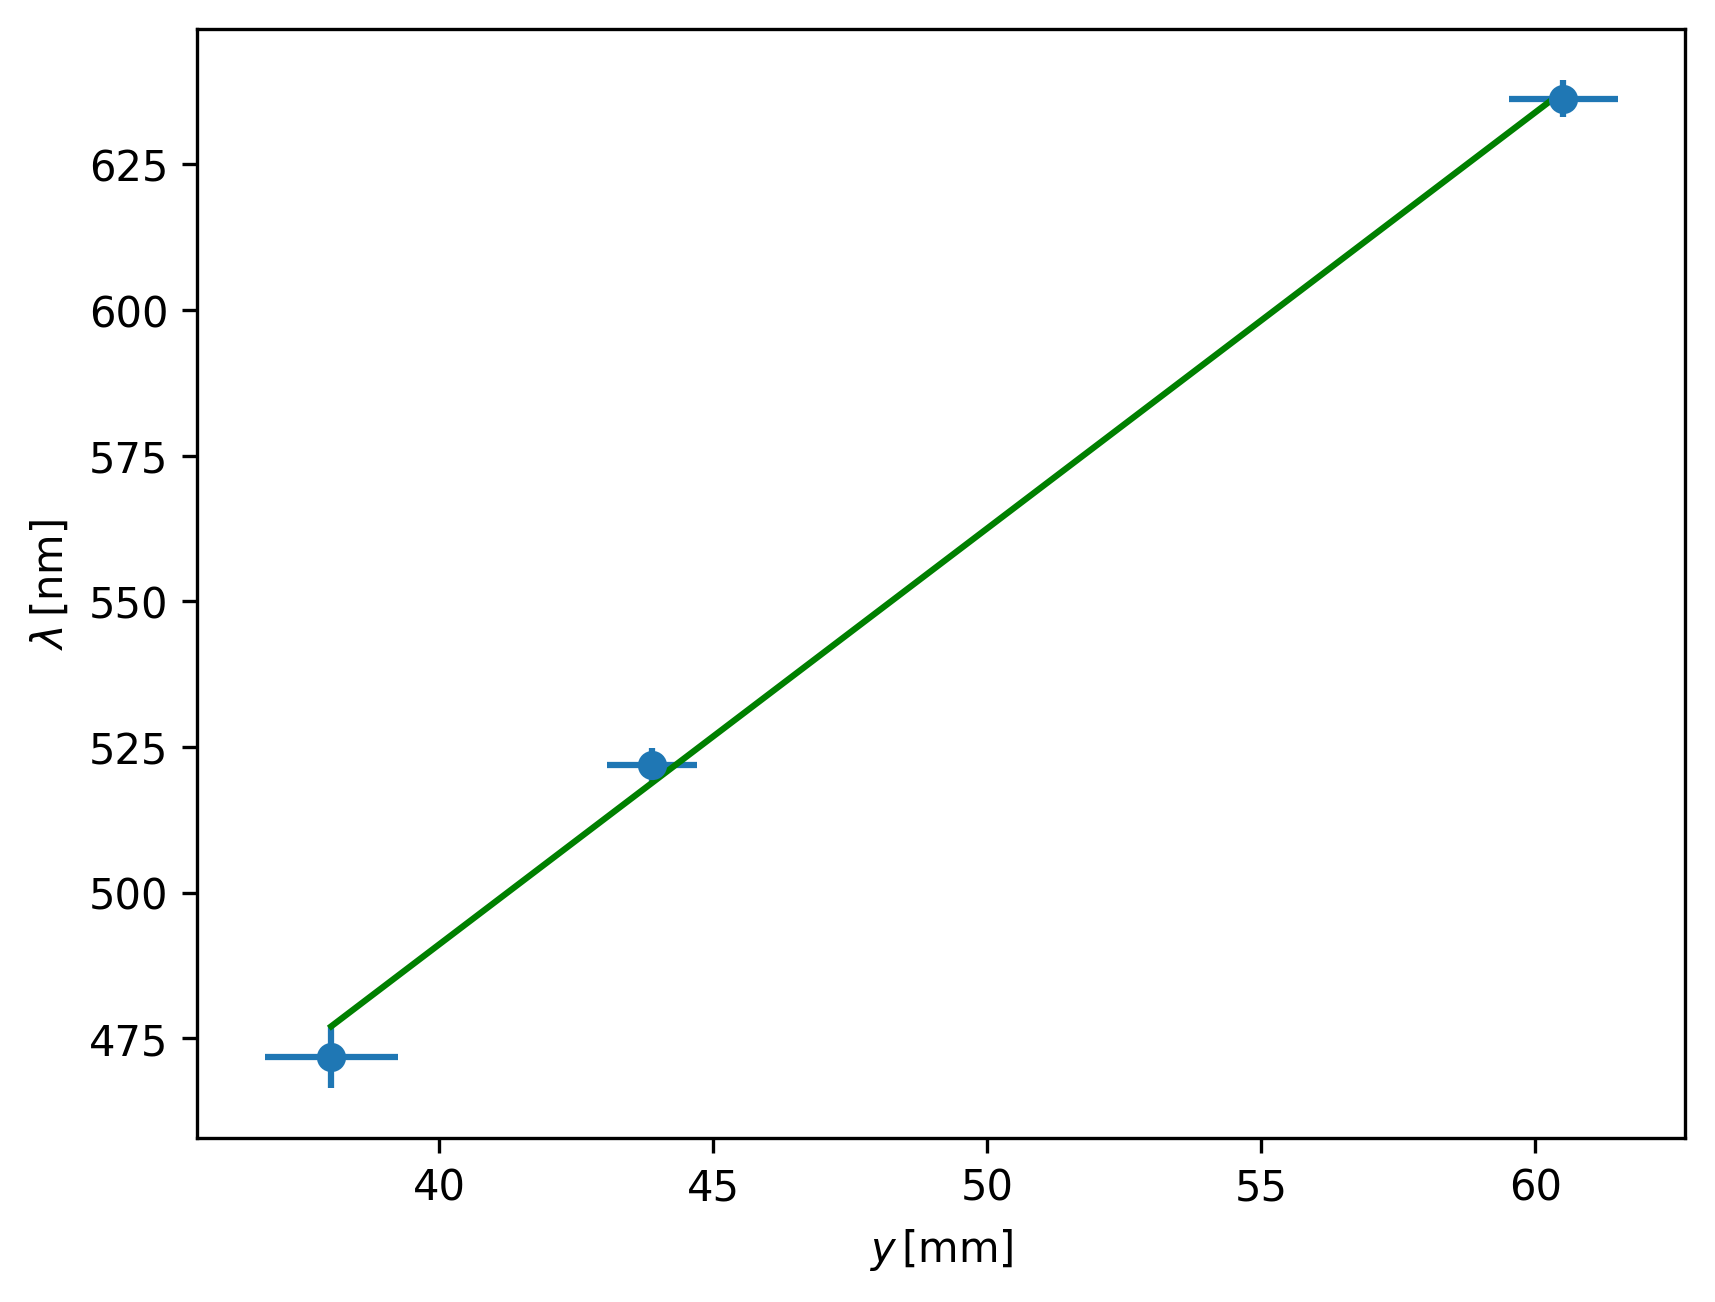
\includegraphics[width=\linewidth]{line_fit_wavelength_1}
    \caption{seria 2}
    \label{fig:line_fit_wavelength_2}
  \end{subfigure}
  \caption{Dopasowanie liniowe \(y(\lambda)\).}
  \label{fig:line_fit_wavelength}
\end{figure}

\textbf{Seria 1 (rys.~\ref{fig:line_fit_wavelength_1}):}  
\(A = (7{,}29 \pm 0{,}53) \times 10^{-6}, \quad B = (-202 \pm 24)\,\mathrm{nm},\)

\[
  \text{macierz kowariancji} =
  \begin{bmatrix}
      2{,}7181 \times 10^{-13} & -1{,}1801 \times 10^{-14}\,\mathrm{m} \\
    -1{,}1801 \times 10^{-14}\,\mathrm{m} & 5{,}3402 \times 10^{-16}\,\mathrm{m}^2
  \end{bmatrix}.
\]

\textbf{Seria 2 (rys.~\ref{fig:line_fit_wavelength_2}):}  
\(A = (7{,}14 \pm 0{,}37) \times 10^{-6}, \quad B = (-205 \pm 18)\,\mathrm{nm},\)

\[
  \text{macierz kowariancji} =
  \begin{bmatrix}
    1{,}3420 \times 10^{-13} & -6{,}4788 \times 10^{-15}\,\mathrm{m} \\
    -6{,}4788 \times 10^{-15}\,\mathrm{m} & 3{,}2338 \times 10^{-16}\,\mathrm{m}^2
  \end{bmatrix}.
\]

Średnia ważona:  
\[
    A = (7{,}19 \pm 0{,}30) \times 10^{-6}, \quad
      B = (-204 \pm 15)\,\mathrm{nm}.
\]

\subsection*{Źródła niepewności}

Błędy pomiaru mogą wynikać z kilku czynników.  
Po pierwsze, układ optyczny został początkowo zestrojony do lasera; po zastąpieniu źródła lampą RGB konieczne było ponowne ustawienie soczewek, lecz nie udało się uzyskać pełnego ogniskowania.  
Po drugie, natężenie sygnału padającego na detektor było niskie, co uwydatniło ograniczenia czułości urządzenia przy wyznaczaniu maksimów.  
Niepewność spektrometru komercyjnego jest natomiast pomijalnie mała w porównaniu z wymienionymi efektami.

\newpage
\begin{thebibliography}{1}

\bibitem{skrypt}
\emph{Budowa i kalibracja spektrometru}, A.~Drabińska, Uniwersytet Warszawski.

\end{thebibliography}

\end{document}
